%% INSTALLATIEHANDLEIDING
\chapter{Installatiehandleiding}
\label{ch:installatiehandleiding}
Dit hoofdstuk bespreekt hoe het software-pakket lokaal op een toestel kan 
draaien. De volgende logingegevens kunnen gebruikt worden om te authenticeren op de applicatie:

\begin{table}[ht]
 \centering
 \begin{tabular}{l | l | l}
    username & passwoord & rol \\
    \hline
    docent & test & docent \\
    student & test & student
 \end{tabular}
\end{table}





\section{Hardware en Software}
\label{sec:hardware_and_software}
De applicatie kan op volgende besturingssystemen draaien:
\begin{itemize}
	\item Linux (32 en 64 bit)
	\item macOS (64 bit)
	\item Windows 7 of hoger (32 en 64 bit)
\end{itemize}

Verder moeten ook nog volgende softwarepakketten ge\"installeerd worden.
\begin{itemize}
\item Node.js (minimum v8.9.4): \url{https://nodejs.org/en/download/}. Opteer voor het 
\textit{.msi} bestand voor Windows en het .pkg bestand voor macOS zoals te zien op figuur \ref{fig:node_1} om de installatieprocedure zo eenvoudig 
mogelijk uit te voeren. Controleer of dit juist ge\"installeerd is door het commando \texttt{node -v} uit te voeren in een terminal of console.
\begin{figure}[ht]
        \centering
 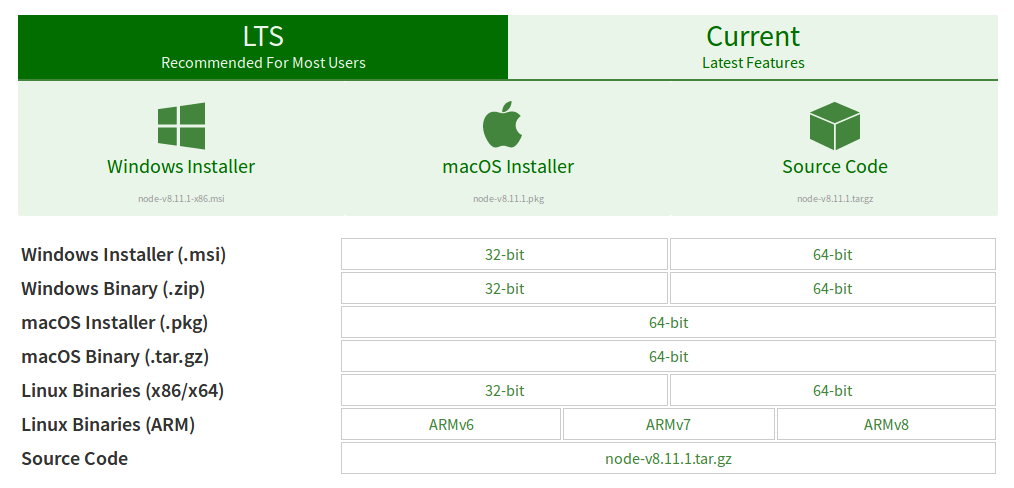
\includegraphics[width=0.9\textwidth]{install_guide/node_1}
 \caption{Node pagina - download}
 \label{fig:node_1}

\end{figure}
\item MongoDB (minimum v2.6.10): \url{https://www.mongodb.com/download-center} 
en klik op \texttt{Community Server} zoals aangegeven in figuur \ref{fig:mongo_1}.
\begin{figure}[ht]
\centering
 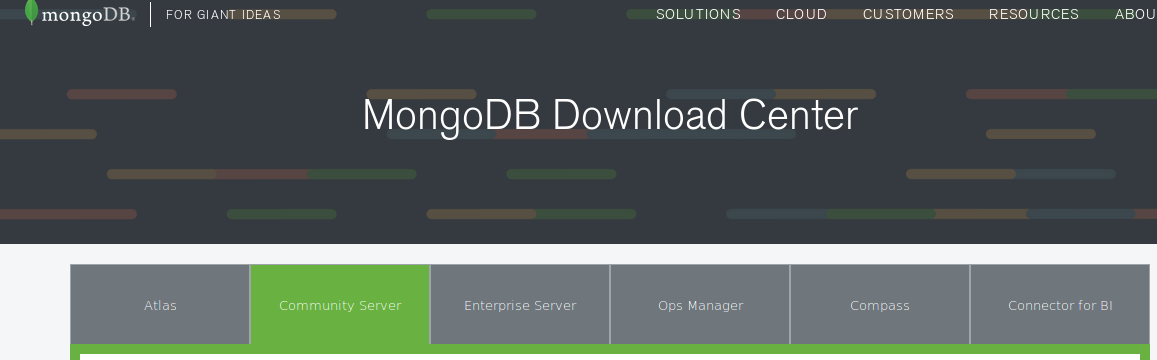
\includegraphics[width=0.9\textwidth]{install_guide/mongo_1}
 \caption{Mongo pagina - Community Server}
 \label{fig:mongo_1}
\end{figure}
Klik vervolgens op het gewenste besturingssysteem en klik dan op download zoals te zien op figuur \ref{fig:mongo_2}. Controleer of dit juist ge\"installeerd is door het commando \texttt{mongo  --version} uit te voeren in een terminal of console.
\begin{figure}[ht]
\centering
 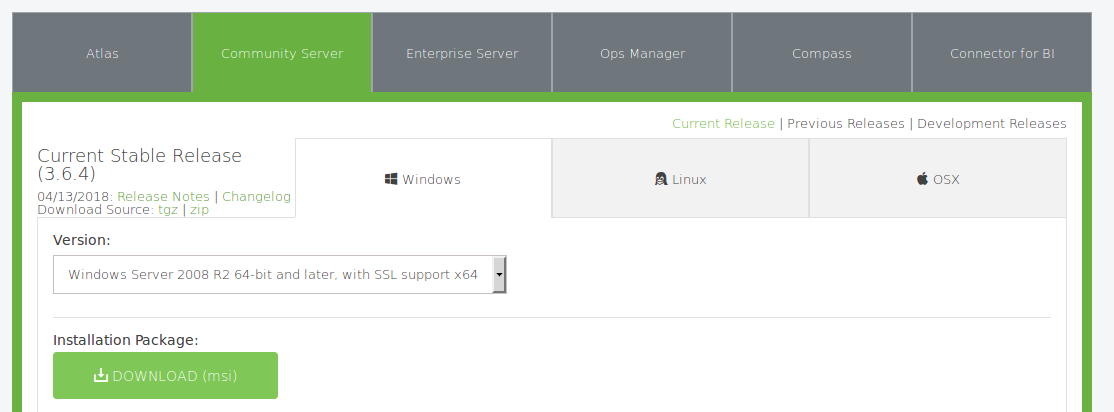
\includegraphics[width=0.9\textwidth]{install_guide/mongo_2}
 \caption{Mongo pagina - download}
 \label{fig:mongo_2}
\end{figure}

    \item Java 8 (minimum $JDK\;8u171$): \url{https://www.java.com/en/download/win10.jsp} : Klik op de download knop en volg de installatieprocedure. Controleer of dit juist ge\"installeerd is door het commando \texttt{java --version} uit te voeren in een terminal of console.
    
    \item ffmpeg : Dit bevat enkel builds voor Windows en macOS. Een .bz2 bestand kan teruggevonden worden op \url{https://ffmpeg.org/download.html}. Om te controleren of dit programma correct is geïnstalleerd kan het commando \texttt{ffmpeg} uitgevoerd worden in de console of terminal.

\end{itemize}

\section{Downloaden repository}
\label{sec:download_repository}
Nadat al de benodigde software ge\"installeerd is moet de broncode op het toestel geplaatst worden. Dit kan op twee manieren:
\begin{enumerate}
    \item Indien \textit{git} ge\"installeerd is op het toestal kan het commando 
    
    \texttt{git clone https://github.ugent.be/bp-vop-2018/annotatietool-01.git} 
    
    gebruikt worden. Dit zal een folder aanmaken met de naam \texttt{annotatietool-01} waarin de broncode terug te vinden is.
    
    \item Indien het toestel geen \textit{git}  heeft, kan de repository nog altijd manueel gedownload worden via \url{https://github.ugent.be/bp-vop-2018/annotatietool-01}. Klik op 
\texttt{Clone or download} en dan \texttt{Download ZIP} zoals te zien op figuur \ref{fig:git_1}. Dit zal een ZIP 
bestand downloaden waarin de broncode terug te vinden is. Plaats de inhoud van het ZIP bestand (folder genaamd \texttt{annotatietool-01}) op het toestel.
\begin{figure}[ht]
 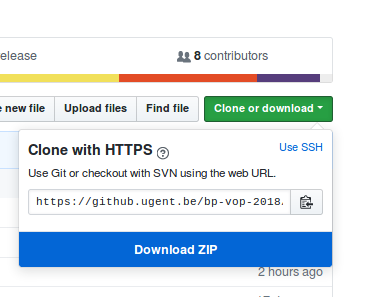
\includegraphics[width=0.5\textwidth]{install_guide/git_1}
 \centering
 \caption{Github pagina : download}
 \label{fig:git_1}
\end{figure}
\end{enumerate}

\subsection{Structuur repository}
Al de broncode van het project bevindt zich in \texttt{annotatietool-01}. De belangrijkste items in deze folder zijn:
\begin{itemize}
 \item \textbf{app.js} : Dit bestand is het startpunt van de applicatie.
 \item \textbf{src}    : Deze folder bevat alle code in verband met de frontend.
 \item \textbf{backend} : Deze folder bevat all code met betrekking tot de backend.
 \item \textbf{spec}    : Deze folder bevat integratietesten voor de webapplicatie (zie \ref{sec:test_exec_web} om de testen uit te voeren).
 \item \textbf{java}    : Deze folder bevat het java-gedeelte van het project (de MP4 converter). De unit testen zitten ook in deze folder (zie \ref{sec:test_exec_java} om de testen uit te voeren).
\end{itemize}




\section{Runnen applicatie}
\label{sec:run_app}
Er bestaan twee mogelijkheden om de applicatie te draaien op een lokaal toestel. 
\subsubsection{Docker}
Hiervoor moet Docker ge\"installeerd worden op het toestel. Navigeer naar \url{https://store.docker.com/search?type=edition&offering=community} om naar een lijst te gaan van de community edition van Docker per besturingssysteem. Kies de versie dat past bij het besturingssysteem van het toestel en voer de installatieprocedure uit.

Indien Docker ge\"installeerd is op het toestel kan het commando \texttt{./buildandrun.sh} uitgevoerd worden in de root directory van het project (annotatietool-01).
Als de docker frontend container in productie gedeployed wordt, dan moet de \texttt{ --disable-host-check} flag verwijdert worden uit de Dockerfile, alsook moet de host gespecifieerd worden voor de productieomgeving.
De webapplicatie kan vanaf nu bediend worden op het lokaal adres \texttt{localhost:9000} via een webbrowser.
\subsubsection{Zonder docker}
Indien geen gebruik gemaakt wordt van docker moet de technologiestack 
zelfstandig ge\"installeerd worden. Voer volgende stappen uit.
\begin{enumerate}
	\item Navigeer naar de \texttt{project} folder (annotatie-tool-01/project).
	\item Open een terminal of de console (afhankelijk van het besturingssysteem) 
	      en voer het commando \texttt{npm install} uit. Dit zal alle nodige 
	      afhankelijkheden van het project laden.
	\item Wanneer alle afhankelijkheden geladen zijn, kan het commando \texttt{npm 
	start} uitgevoerd worden. Dit zal de backend opstarten met als onderliggende 
	commando \texttt{ng build \&\& nodemon www.js}. Het defaultadres van de backend 
	is \texttt{localhost:3000}. Figuur \ref{fig:npm_start_ex} toont 
	voorbeelduitvoer van dit commando.
	\begin{figure}[ht]

		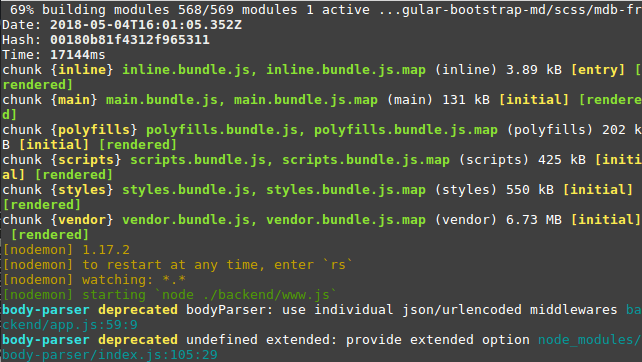
\includegraphics[width=\textwidth]{npm_start_ex}  		
		\caption{Uitvoer van \texttt{npm start} op een linux toestel}
		\label{fig:npm_start_ex}
	\end{figure}
	
	\item Open een nieuwe terminal of console en voer het commando \texttt{ng 
	serve} uit. Dit zal de webapplicatie lokaal starten. Dit commando zal zeggen op 
	welk adres de applicatie draait. Het defaultadres is \texttt{localhost:4200}. 
	Figuur \ref{fig:ng_serve_ex} toont voorbeelduitvoer van dit commando.
	\begin{figure}[ht]
		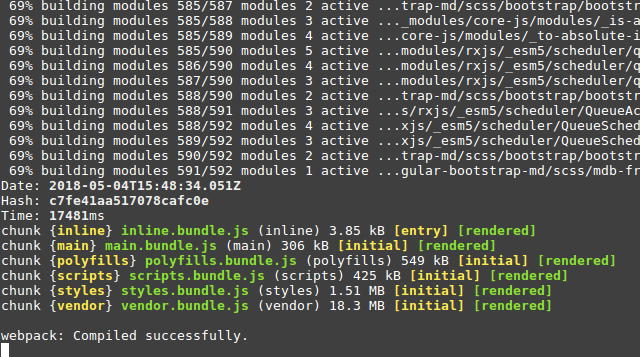
\includegraphics[width=\textwidth]{ng_serve_ex}  
		
		\caption{Uitvoer van \texttt{ng serve} op een linux toestel}
		\label{fig:ng_serve_ex}
	\end{figure}
	
	
	\item Navigeer in een webbrowser naar \texttt{localhost:4200} om de 
	      applicatie te bedienen.
\end{enumerate}



    
\section{Het uitvoeren van testen}
\label{sec:test_exec}
Er zijn twee luiken van testen. Het eerste luik test de operaties die 
worden gebruikt door de webapplicatie. Het tweede luik zijn de JUnit testen voor 
de MP4 Converter.
    
\subsection{Testen van de webapplicatie}
\label{sec:test_exec_web}
De benodigde software is voor dit luik al ge\"installeerd indien de vorige secties correct uitgevoerd zijn. Start de applicatie zoals beschreven in \ref{sec:run_app} en navigeer naar de folder \texttt{annotatietool-01/project} en voer het commando \texttt{npm test} uit. Indien de testen correct zijn uitgevoerd wordt de output van figuur \ref{fig:web_tests} weergegeven.
\begin{figure}[ht]
	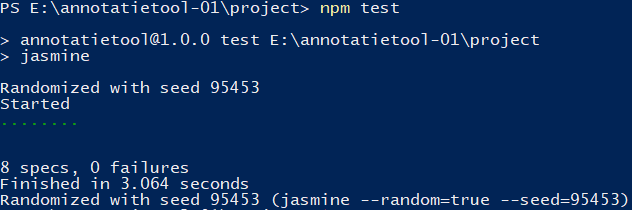
\includegraphics[width=\textwidth]{web_tests}  
	\caption{De uitvoer van correct uitgevoerde integratietesten}
    \label{fig:web_tests}
\end{figure}
\subsection{Testen van de MP4 Converter}
\label{sec:test_exec_java}
Aangezien de MP4 Converter geschreven is in Java is het logisch dat de testsuites geschreven zijn met behulp van JUnit. Indien sectie \ref{sec:hardware_and_software} correct uitgevoerd is, kunnen de JUnit testen uitgevoerd worden. Navigeer vanuit de root folder naar \texttt{java/MP4Converter/} en voer het volgende commando uit:
\texttt{java -jar RunTests.jar}. Om te weten dat alle tests correct uitgevoerd worden zou de output van figuur \ref{fig:java_tests} tevoorschijn moeten komen.
\begin{figure}[ht]
	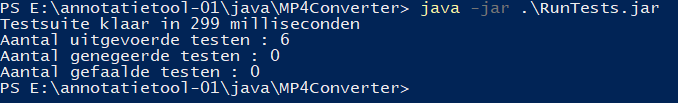
\includegraphics[width=\textwidth]{java_tests}  
	\caption{De uitvoer van correct uitgevoerde JUnit testen}
    \label{fig:java_tests}
\end{figure}

